% TikZ Diagram: GPS Orbit Geometry with Time Dilation
% Pedagogical visualization showing Earth, GPS satellite orbit, and gravitational effects
% Style inspired by Lions Commentary clarity

\begin{figure}[htbp]
\centering
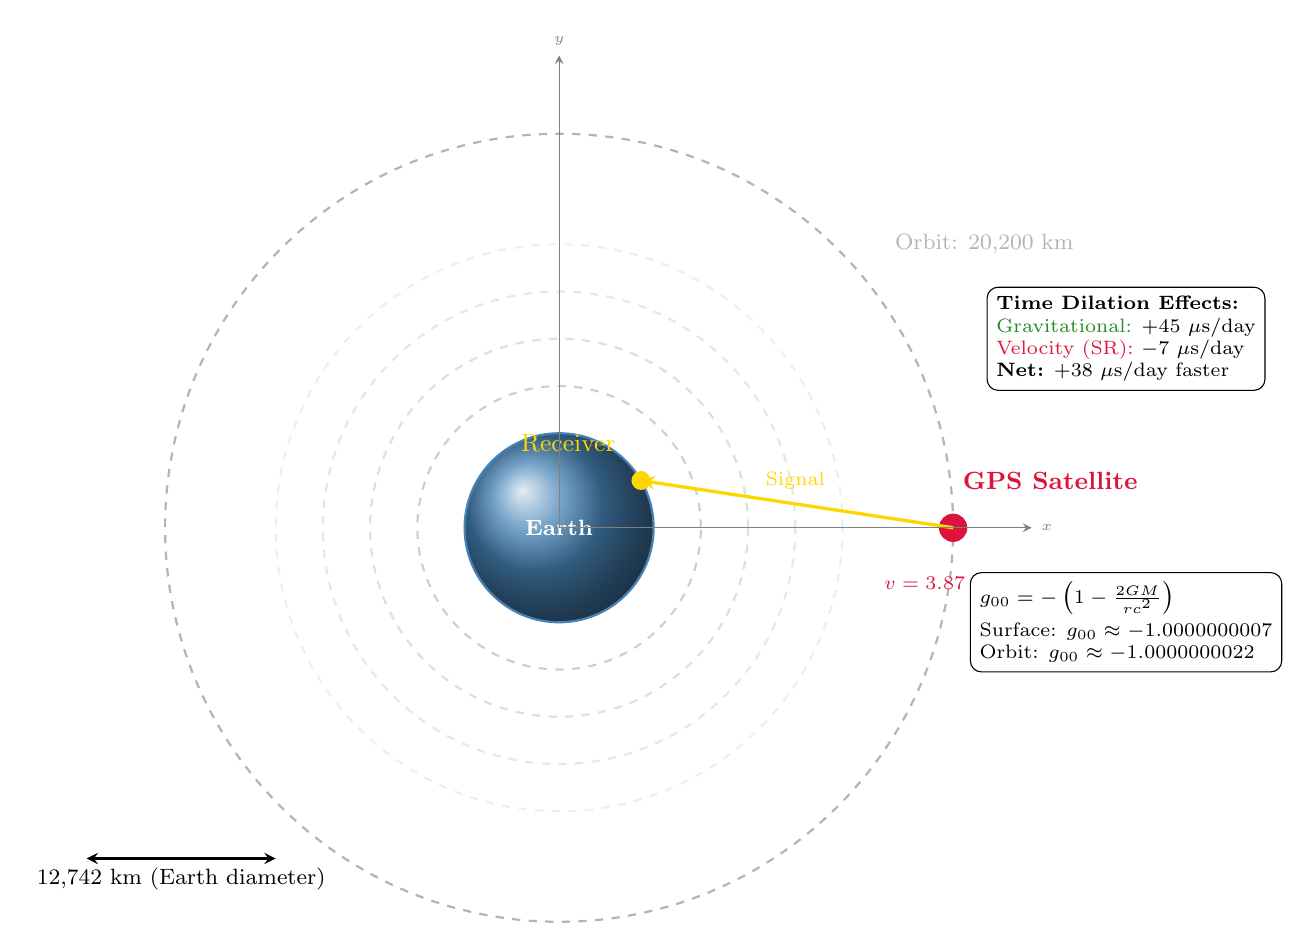
\begin{tikzpicture}[scale=1.2, >=stealth]
  
  % Define colors
  \definecolor{earthblue}{RGB}{70,130,180}
  \definecolor{orbitgray}{RGB}{180,180,180}
  \definecolor{satred}{RGB}{220,20,60}
  \definecolor{potentialgreen}{RGB}{34,139,34}
  \definecolor{signalgold}{RGB}{255,215,0}
  
  % Earth (radius normalized to 1 unit = 6371 km)
  \shade[ball color=earthblue] (0,0) circle (1);
  \draw[thick, earthblue] (0,0) circle (1);
  \node at (0,0) {\footnotesize \textcolor{white}{\textbf{Earth}}};
  
  % Gravitational potential contours
  \foreach \r/\opacity in {1.5/0.3, 2.0/0.2, 2.5/0.15, 3.0/0.1} {
    \draw[potentialgreen, opacity=\opacity, dashed, thick] (0,0) circle (\r);
  }
  
  % GPS orbit (altitude 20,200 km → radius 4.17 Earth radii)
  \draw[thick, orbitgray, dashed] (0,0) circle (4.17);
  \node[orbitgray] at (4.5, 3) {\footnotesize Orbit: 20,200 km};
  
  % GPS satellite
  \fill[satred] (4.17, 0) circle (0.15);
  \node[satred, above right] at (4.17, 0.3) {\small \textbf{GPS Satellite}};
  \node[satred, below] at (4.17, -0.4) {\scriptsize $v = 3.87$ km/s};
  
  % Ground receiver
  \fill[signalgold] (0.866, 0.5) circle (0.1);  % At 30° on surface
  \node[signalgold, above left] at (0.7, 0.7) {\small Receiver};
  
  % Signal path
  \draw[signalgold, very thick, ->] (4.17, 0) -- (0.866, 0.5);
  \node[signalgold] at (2.5, 0.5) {\scriptsize Signal};
  
  % Time dilation annotations
  \node[draw, fill=white, rounded corners, align=left, font=\scriptsize] at (6, 2) {
    \textbf{Time Dilation Effects:}\\
    \textcolor{potentialgreen}{Gravitational:} $+45$ $\mu$s/day\\
    \textcolor{satred}{Velocity (SR):} $-7$ $\mu$s/day\\
    \textbf{Net:} $+38$ $\mu$s/day faster
  };
  
  % Metric annotation
  \node[draw, fill=white, rounded corners, align=left, font=\scriptsize] at (6, -1) {
    $g_{00} = -\left(1 - \frac{2GM}{rc^2}\right)$\\[2pt]
    Surface: $g_{00} \approx -1.0000000007$\\
    Orbit: $g_{00} \approx -1.0000000022$
  };
  
  % Scale bar
  \draw[<->, thick] (-5, -3.5) -- (-3, -3.5);
  \node[below] at (-4, -3.5) {\footnotesize 12,742 km (Earth diameter)};
  
  % Coordinate axes
  \draw[->, gray] (0,0) -- (5, 0) node[right] {\tiny $x$};
  \draw[->, gray] (0,0) -- (0, 5) node[above] {\tiny $y$};
  
\end{tikzpicture}
\caption{GPS satellite orbit geometry showing gravitational time dilation effects. The satellite at 20,200 km altitude experiences weaker gravitational field (lighter green contours) than Earth's surface, causing its clock to run faster by $+45$ $\mu$s/day. Combined with special relativistic velocity time dilation ($-7$ $\mu$s/day), the net effect is $+38$ $\mu$s/day faster. Without correction, position errors accumulate at $\approx 11$ km/day, making Einstein's equations essential for navigation.}
\label{fig:prelim:gps-orbit-detailed}
\end{figure}
